\section{The CPR Toolkit}

The Comprehensible Provenance Record (CPR) Toolkit is a suite of tools for recording, storing, querying, and visualizing the provenance of artifacts produced by a run of a computational workflow. As the name suggests, a key objective of the toolkit is to make provenance easily comprehensible, not to systems programmers, but rather to practitioners of a research domain seeking to understand how the computational artifacts associated with a study in that domain were obtained.

While the primary purpose of CPR at present is to automate the monitoring and management of provenance-relevant events and records associated with a Whole Tale \emph{recorded run}, the toolkit can be deployed in any Linux-based computing environment and used to capture, query, and reason about provenance of computational artifacts produced in that environment.

CPR employs \programname{ReproZip} \cite{rampin_reprozip_2016} to observe system calls invoked as part of the recorded run and to record metadata about (1) the operating-system level processes comprising the overall computation; (2) the files accessed by these processes; and (3) the access mode for file accesses, i.e. whether processes opened files for reading, writing, or both. \programname{ReproZip} captures and records all of this information in a SQLite database with a schema specific to ReproZip.

Once a recorded run is complete, the \programname{cpr} command-line utility extracts these OS-level records from the ReproZip trace, transform them into RDF triples, and loads the triples into an RDF dataset in an instance of Blazegraph. The triples are expressed using a vocabulary developed to represent provenance information in the context of Whole Tale recorded run executions (Figure \ref{fig:cpr-vocab}). 

\begin{figure}[h]
    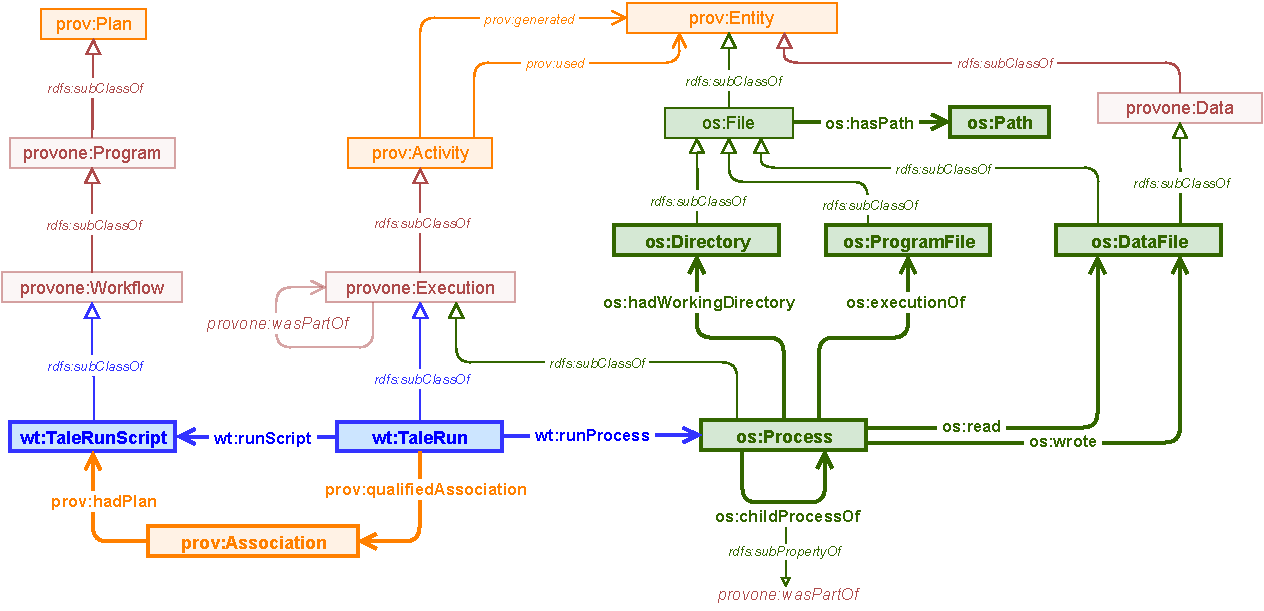
\includegraphics[width=\linewidth]{figures/cpr-vocab.pdf}
    \caption{Relationship of key elements of the CPR vocabulary to classes and properties defined by the PROV and ProvONE vocabularies.}
    \label{fig:cpr-vocab}
\end{figure}

The CPR vocabulary extends PROV and ProvONE \cite{provone_2015} with subclasses specific to Whole Tale to unambiguously represeent run-time provenance records captured from multiple recorded runs and distinct versions of a particular Tale. CPR can represent this vocabulary either as Datalog facts or as RDF triples. Because Blazegraph provides an eager reasoner, all triples implied by the subclass relationships are generated automatically when loading a CPR trace into Blazegraph. Consequently, a CPR trace, asserted using the CPR vocabulary, can be queried in terms of the PROV and ProvONE vocabularies, without using a reasoner at query time.

The CPR toolkit and vocabulary recognize the distinct roles played by particular files during a run. A simple YAML file is used to declare a run profile that associates roles with individual files, particular directories, or entire directory trees. Using these declarations while converting a ReproZip trace to the CPR vocabulary, the toolkit is able to distinguish data files of scientific significance from, e.g., shared libraries associated with the operating system or provided by software dependencies, and automatically mask these (often numerous) files in queries and visualization by default.

Finally, the Geist report-templating tool is used to pose SPARQL queries against the Blazegraph instance, to format the query results as reports, and to create visualizations of query results using Graphviz.  Geist queries, reports, and visualizations may be parameterized. In Whole Tale we plan to create a predefined set of reports and visualizations following each recorded run.
